% Op icon: hole — block cross-section with a plain drilled channel through it.
\documentclass[tikz,border=2mm]{standalone}
\usetikzlibrary{arrows.meta,calc,shapes.geometric}
\begin{document}
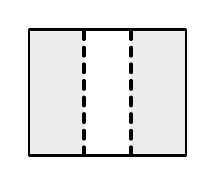
\begin{tikzpicture}[line width=1.3pt, line cap=round, line join=round, >=Stealth, x=1mm,y=1mm]
  % Fill the block MINUS the channel as one compound (even-odd) path, rather
  % than punching a `\fill[white]` hole over it — a literal white fill would
  % show as a solid white block against this button's actual (non-white,
  % theme-dependent) background instead of reading as empty space.
  \fill[gray!15, even odd rule] (-10,-8) rectangle (10,8) (-3,-8) rectangle (3,8);
  \draw[thick] (-10,-8) rectangle (10,8);
  \draw[dashed] (-3,-8) -- (-3,8);
  \draw[dashed] (3,-8) -- (3,8);
\end{tikzpicture}
\end{document}
